On considère la fonction $f$ définie sur $\R$ par \[f(x) = x^3\e^x.\]
%
On admet que la fonction $f$ est dérivable sur $\R$ et on note $f'$ sa fonction dérivée.

\begin{enumerate}
	\item On définit la suite $\left(u_n\right)$ par $u_0 = - 1$ et, pour tout entier naturel $n$, $u_{n+1} = f\left(u_n\right)$.
	\begin{enumerate}
		\item Calculer $u_1$  puis $u_2$.
		
		On donnera les valeurs exactes, puis les valeurs approchées à $10^{-3}$.
		\item On considère la fonction \texttt{fonc}, écrite en langage \textsf{Python} ci-dessous.
		
		\smallskip
		
		On rappelle qu'en langage \textsf{Python}, \texttt{i in range(n)} signifie que \texttt{i} varie de \texttt{0} à \texttt{n-1}.
		%
\begin{CodePythonLstAlt}*[Largeur=8cm]{center}
def fonc(n) :
	u = -1
	for i in range(n) :
		u = u**3 * exp(u)
	return u
\end{CodePythonLstAlt}
		%
		Déterminer, sans justifier, la valeur renvoyée par \texttt{fonc(2)} arrondie à $10^{-3}$.
	\end{enumerate}
	\item 
	\begin{enumerate}
		\item Démontrer que, pour tout $x$ réel, on a $f'(x) = x^2\e^x(x + 3)$.
		\item Justifier que le tableau de variations de $f$ sur $\R$ est celui représenté ci-dessous :
		
		\begin{center}
			\begin{tikzpicture}
				\tkzTabInit{$x$/1,$f$/2}{$-\infty$,$-3$,$+\infty$}
				\tkzTabVar{+/$0$,-/$- 27\e^{-3}$,+/$+\infty$}
			\end{tikzpicture}
		\end{center}
		\item Démontrer, par récurrence, que pour tout entier naturel $n$, on a : \[- 1 \leqslant u_n \leqslant u_{n+1} \leqslant 0.\]
		\item En déduire que la suite $\left(u_n\right)$ est convergente.
		\item On note $\ell$ la limite de la suite $\left(u_n\right)$.
		
		On rappelle que $\ell$ est solution de l'équation $f(x) = x$.
		
		Déterminer $\ell$. Pour cela, on admettra que l'équation $x^2\e^x - 1 = 0$ possède une seule solution dans $\R$ et que celle-ci est strictement supérieure à $\dfrac12$).
	\end{enumerate}
\end{enumerate}

